\documentclass[12pt, a4paper]{article}

% ── Packages ──
\usepackage[utf8]{inputenc}
\usepackage[T1]{fontenc}
\usepackage{lmodern}
\usepackage[margin=2.5cm]{geometry}
\usepackage{graphicx}
\usepackage{xcolor}
\usepackage{tikz}
\usetikzlibrary{shapes.geometric, arrows.meta, positioning, fit, calc, backgrounds, decorations.pathreplacing}
\usepackage{booktabs}
\usepackage{tabularx}
\usepackage{multirow}
\usepackage{enumitem}
\usepackage{hyperref}
\usepackage{fancyhdr}
\usepackage{titlesec}
\usepackage{float}
\usepackage{caption}
\usepackage{subcaption}
\usepackage{amsmath}
\usepackage{parskip}

% ── Colors ──
\definecolor{inmindteal}{HTML}{00D4AA}
\definecolor{inmindpurple}{HTML}{7C3AED}
\definecolor{inmindblue}{HTML}{0284C7}
\definecolor{inmindpink}{HTML}{DB2777}
\definecolor{darkbg}{HTML}{0A0A12}
\definecolor{sectioncolor}{HTML}{1E3A5F}

% ── Hyperref setup ──
\hypersetup{
    colorlinks=true,
    linkcolor=sectioncolor,
    urlcolor=inmindblue,
    citecolor=inmindpurple,
}

% ── Header / Footer ──
\pagestyle{fancy}
\fancyhf{}
\fancyhead[L]{\small\textcolor{gray}{ITIP Progress Report}}
\fancyhead[R]{\small\textcolor{gray}{Carl Wakim — Spring 2026}}
\fancyfoot[C]{\thepage}
\renewcommand{\headrulewidth}{0.4pt}

% ── Section styling ──
\titleformat{\section}{\Large\bfseries\color{sectioncolor}}{}{0em}{}[\titlerule]
\titleformat{\subsection}{\large\bfseries\color{sectioncolor!80}}{}{0em}{}

% ── Title ──
\title{
    \vspace{-1cm}
    {\LARGE\bfseries InMind Talent Intelligence Platform (ITIP)}\\[0.3cm]
    {\Large Progress Report — Gen AI Track}\\[0.2cm]
    {\large Spring 2026}
}
\author{Carl Wakim}
\date{March 2026}

\begin{document}

\maketitle
\thispagestyle{fancy}

% ══════════════════════════════════════════════════════════
\begin{abstract}
This report presents the progress on the InMind Talent Intelligence Platform (ITIP), a production-oriented multi-agent AI system for talent acquisition and BMW placement intelligence. The platform features a six-container Docker architecture comprising two independent agent systems (LangGraph and Google ADK), a vector-database-backed RAG pipeline, role-based access control, input/output guardrails, a fine-tuned DistilBERT track classifier, and MCP-based interview scheduling tools. The system is fully functional with synthetic data, achieving 96.55\% routing accuracy, 88.5\% RAGAS faithfulness, and 97\% classifier accuracy. Remaining work includes production PDF ingestion and Whisper-based voice interface testing.
\end{abstract}

\tableofcontents
\newpage

% ══════════════════════════════════════════════════════════
\section{Introduction}

The InMind Talent Intelligence Platform (ITIP) is a multi-agent AI system designed to support talent acquisition workflows at inmind.ai, including candidate screening, job search, HR policy lookup, and BMW Group internship placement management.

The platform serves four distinct user roles — job seekers, HR recruiters, InMind staff, and academy instructors — each with tailored access to specialized AI agents. The system combines retrieval-augmented generation (RAG), skill-weighted candidate matching, classification via fine-tuned DistilBERT, and tool-use through the Model Context Protocol (MCP).

\subsection{Objectives}

\begin{itemize}[leftmargin=1.5em]
    \item Build a multi-agent system using two distinct frameworks (LangGraph and Google ADK)
    \item Implement RAG over four domain-specific corpora with per-corpus chunking strategies
    \item Provide role-based access control with input/output guardrails
    \item Fine-tune a DistilBERT classifier for BMW internship track prediction
    \item Expose interview scheduling tools via MCP protocol
    \item Containerize the full stack with Docker Compose
    \item Evaluate with retrieval metrics, RAGAS, routing accuracy, and classifier metrics
\end{itemize}

% ══════════════════════════════════════════════════════════
\section{System Architecture}

The platform follows a six-container microservices architecture. All inter-service communication occurs via HTTP — no shared Python imports between services.

\begin{figure}[H]
\centering
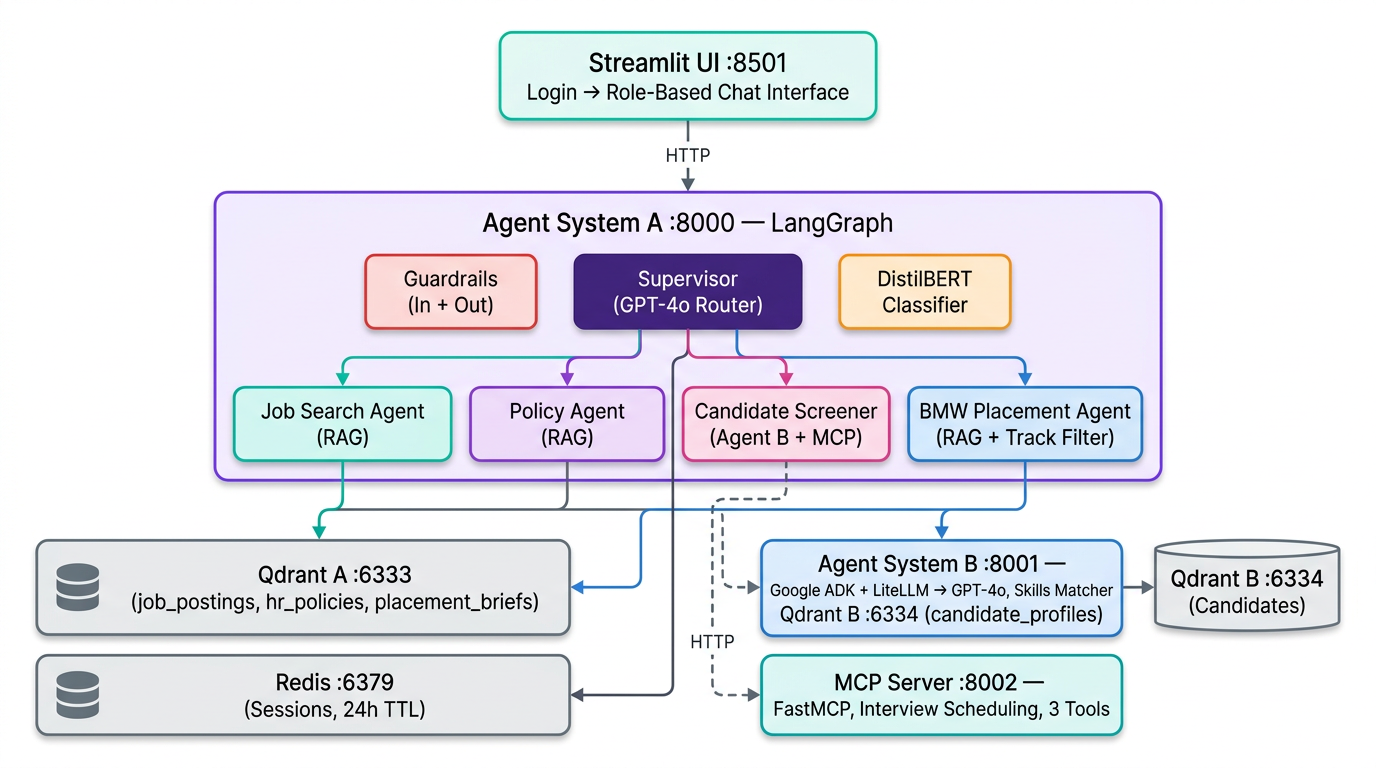
\includegraphics[width=\textwidth]{itip_architecture.png}
\caption{ITIP System Architecture — six-container microservices stack}
\label{fig:architecture}
\end{figure}

\begin{table}[H]
\centering
\caption{Container summary}
\begin{tabularx}{\textwidth}{l l l X}
\toprule
\textbf{Container} & \textbf{Port} & \textbf{Framework} & \textbf{Purpose} \\
\midrule
Agent System A & 8000 & FastAPI + LangGraph & Supervisor + 4 specialists, guardrails, DistilBERT, voice \\
Agent System B & 8001 & FastAPI + Google ADK & Skills matching with embedding similarity + skill scoring \\
MCP Server & 8002 & FastAPI + FastMCP & Interview scheduling tools (mock data) \\
Qdrant A & 6333 & Qdrant & Job postings, HR policies, placement briefs \\
Qdrant B & 6334 & Qdrant & Candidate profiles \\
Redis & 6379 & Redis & Conversation session storage (24h TTL) \\
\bottomrule
\end{tabularx}
\label{tab:containers}
\end{table}

% ══════════════════════════════════════════════════════════
\section{Agent System A — LangGraph Supervisor}

Agent System A is the primary entry point for all user interactions. It implements a \textbf{supervisor-specialist pattern} using LangGraph, where a GPT-4o-based supervisor classifies user intent and routes to one of four specialist agents.

\subsection{Supervisor Agent}

The supervisor receives the user's message along with conversation history and outputs a JSON routing decision. It operates at \texttt{temperature=0.0} for deterministic classification. The supervisor also enforces role-based access — if the selected specialist is outside the user's allowed list, the request is blocked with an explanatory message.

Available routes: \texttt{job\_search}, \texttt{policy}, \texttt{candidate\_screener}, \texttt{bmw\_placement}, and \texttt{FINISH}.

\subsection{Specialist Agents}

\begin{figure}[H]
\centering
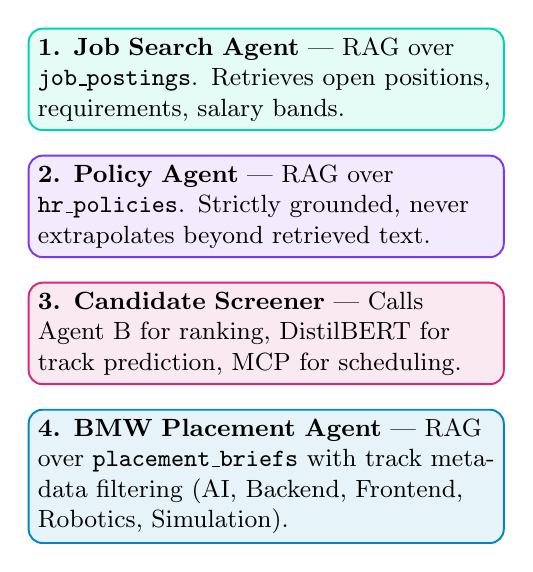
\begin{tikzpicture}[
    node distance=0.4cm,
    every node/.style={font=\small},
    specbox/.style={rectangle, rounded corners=5pt, draw=#1, fill=#1!10, minimum width=6cm, minimum height=0.9cm, align=left, line width=0.7pt, text width=5.8cm},
]

\node[specbox=inmindteal] (s1) {\textbf{1. Job Search Agent} — RAG over \texttt{job\_postings}. Retrieves open positions, requirements, salary bands.};
\node[specbox=inmindpurple, below=0.3cm of s1] (s2) {\textbf{2. Policy Agent} — RAG over \texttt{hr\_policies}. Strictly grounded, never extrapolates beyond retrieved text.};
\node[specbox=inmindpink, below=0.3cm of s2] (s3) {\textbf{3. Candidate Screener} — Calls Agent B for ranking, DistilBERT for track prediction, MCP for scheduling.};
\node[specbox=inmindblue, below=0.3cm of s3] (s4) {\textbf{4. BMW Placement Agent} — RAG over \texttt{placement\_briefs} with track metadata filtering (AI, Backend, Frontend, Robotics, Simulation).};

\end{tikzpicture}
\caption{The four specialist agents in Agent System A}
\label{fig:specialists}
\end{figure}

\subsection{Endpoints}

\begin{itemize}[leftmargin=1.5em]
    \item \texttt{POST /chat} — Main conversational endpoint (synchronous)
    \item \texttt{POST /chat/stream} — Server-Sent Events streaming with real-time node updates
    \item \texttt{POST /chat/voice} — Whisper STT $\to$ pipeline $\to$ OpenAI TTS (returns MP3)
    \item \texttt{GET /session/\{id\}} — Retrieve session history (PII-scrubbed)
    \item \texttt{DELETE /session/\{id\}} — Clear session
    \item \texttt{GET /health} — Health check with Qdrant/Redis connectivity status
\end{itemize}

Rate limiting is applied via \texttt{slowapi}: 30 requests/minute on \texttt{/chat}, 5 requests/minute on \texttt{/chat/voice}.

% ══════════════════════════════════════════════════════════
\section{Agent System B — Google ADK Skills Matcher}

Agent System B is an independent microservice built on the \textbf{Google Agent Development Kit (ADK)} with a LiteLLM adapter routing to GPT-4o. It is responsible for skill-weighted candidate ranking.

\subsection{Matching Pipeline}

The matching process follows five sequential steps:

\begin{enumerate}[leftmargin=1.5em]
    \item \textbf{Skill Parsing} — GPT-4o extracts \texttt{must\_have} and \texttt{nice\_to\_have} skills from the job description
    \item \textbf{Query Embedding} — The job description is embedded using \texttt{text-embedding-3-small} (1536 dimensions)
    \item \textbf{Semantic Search} — Top-20 candidates retrieved from Qdrant B by cosine similarity
    \item \textbf{Composite Scoring} — Each candidate receives a composite score:
    \[
    S = 0.4 \times \text{semantic\_score} \times 100 + 0.6 \times \text{skill\_intersection\_score}
    \]
    where skill intersection uses weighted matching (must-have: $3\times$, nice-to-have: $1\times$) with word-boundary regex to avoid false positives (e.g., ``Java'' does not match ``JavaScript'')
    \item \textbf{Summary Generation} — GPT-4o writes a 2--3 sentence recruiter summary per candidate
\end{enumerate}

\subsection{ADK Agent Definition}

The ADK agent registers two \texttt{FunctionTool}s:
\begin{itemize}[leftmargin=1.5em]
    \item \texttt{adk\_parse\_skills} — Extracts skills from a job description
    \item \texttt{adk\_match\_and\_rank} — Runs the complete matching pipeline
\end{itemize}

Shared clients (OpenAI, Qdrant) are injected at startup via a module-level setter function.

% ══════════════════════════════════════════════════════════
\section{MCP Server — Interview Scheduling}

The MCP (Model Context Protocol) server exposes three interview scheduling tools via both the MCP protocol and REST endpoints. It uses in-memory mock data with six fictional interviewers.

\begin{table}[H]
\centering
\caption{MCP Tools}
\begin{tabularx}{\textwidth}{l X}
\toprule
\textbf{Tool} & \textbf{Description} \\
\midrule
\texttt{find\_available\_interviewers} & Returns available interviewers for a given role, date, and optional BMW track filter \\
\texttt{schedule\_interview} & Books an interview, returns confirmation ID, Zoom link, and status \\
\texttt{send\_assessment} & Dispatches a technical assessment with tracking ID, deadline, and link \\
\bottomrule
\end{tabularx}
\label{tab:mcp}
\end{table}

The Candidate Screener in Agent A calls these tools via HTTP when it detects scheduling intent keywords in the user message (e.g., ``book interview'', ``send assessment'').

% ══════════════════════════════════════════════════════════
\section{RAG Pipeline and Data Ingestion}

\subsection{Embedding Model}

All collections use \texttt{text-embedding-3-small} (1536 dimensions, 8191-token context). The same model is used for both ingestion and query-time embedding.

\subsection{Chunking Strategies}

Each corpus uses a tailored chunking strategy aligned with the project proposal:

\begin{table}[H]
\centering
\caption{Per-corpus chunking configuration}
\begin{tabularx}{\textwidth}{l l c c X}
\toprule
\textbf{Corpus} & \textbf{Strategy} & \textbf{Chunk} & \textbf{Overlap} & \textbf{Rationale} \\
\midrule
Job Postings & Structure-aware & 350 tok & 50 tok & Section-specific queries need section-specific chunks \\
HR Policies & Recursive char split & 500 tok & 100 tok & Policy prose has natural paragraph boundaries \\
Placement Briefs & Recursive + metadata & 450 tok & 90 tok & Mixed doc types; metadata enables pre-filtering \\
Candidate Profiles & Fixed-size + skill tags & 400 tok & 80 tok & Semi-structured, dense vocabulary \\
\bottomrule
\end{tabularx}
\label{tab:chunking}
\end{table}

\subsection{Ingestion Modes}

The ingestion script supports two modes:

\begin{itemize}[leftmargin=1.5em]
    \item \textbf{JSONL mode} (current) — Synthetic data generated by GPT-4o: 21 job postings, 9 HR policies, 14 placement briefs, 33 candidate profiles
    \item \textbf{PDF mode} (production) — Reads from \texttt{data/pdfs/} directories with pdfplumber for text extraction, table detection converted to Markdown, and PyMuPDF for image extraction
\end{itemize}

Point IDs are generated using UUID5 hashing, ensuring re-ingestion is idempotent (no duplicate data).

\subsection{Retrieval}

At query time, the user's message is embedded and the top-$K$ chunks are retrieved from Qdrant by cosine similarity. The retrieved chunks are formatted with source metadata and passed as context to GPT-4o. The BMW Placement specialist additionally applies a Qdrant metadata filter when a specific track is detected.

% ══════════════════════════════════════════════════════════
\section{DistilBERT Track Classifier}

A fine-tuned \texttt{distilbert-base-uncased} model classifies candidate text into one of five BMW internship tracks: AI, Backend, Frontend, Robotics, and Simulation.

\subsection{Training Configuration}

\begin{table}[H]
\centering
\caption{Classifier training details}
\begin{tabular}{l l}
\toprule
\textbf{Parameter} & \textbf{Value} \\
\midrule
Base model & \texttt{distilbert-base-uncased} \\
Training samples & 133 (100 BERT snippets + 33 candidate profiles) \\
Classes & 5 (AI, Backend, Frontend, Robotics, Simulation) \\
Validation & 5-fold stratified cross-validation \\
Epochs & 8 \\
Learning rate & $2 \times 10^{-5}$ \\
Max token length & 256 \\
Optimizer & AdamW (weight decay 0.01) \\
Scheduler & Linear warmup (10\% of steps) \\
\bottomrule
\end{tabular}
\label{tab:bert_config}
\end{table}

\subsection{Results}

\begin{table}[H]
\centering
\caption{DistilBERT cross-validation results}
\begin{tabular}{l c c c c}
\toprule
\textbf{Track} & \textbf{Precision} & \textbf{Recall} & \textbf{F1} & \textbf{Support} \\
\midrule
AI & 1.000 & 0.964 & 0.982 & 28 \\
Backend & 0.963 & 0.963 & 0.963 & 27 \\
Frontend & 0.964 & 0.964 & 0.964 & 28 \\
Robotics & 0.929 & 1.000 & 0.963 & 26 \\
Simulation & 1.000 & 0.958 & 0.979 & 24 \\
\midrule
\textbf{Mean Accuracy} & \multicolumn{4}{c}{\textbf{97.01\% $\pm$ 2.78\%}} \\
\textbf{Macro F1} & \multicolumn{4}{c}{\textbf{97.02\%}} \\
\bottomrule
\end{tabular}
\label{tab:bert_results}
\end{table}

The model is loaded lazily on first inference and cached in memory. If model files are not found, the system gracefully falls back without crashing.

% ══════════════════════════════════════════════════════════
\section{Guardrails}

\subsection{Input Guardrails}

Input guardrails are applied \textbf{before} any agent processing occurs:

\begin{table}[H]
\centering
\caption{Input guardrail layers}
\begin{tabularx}{\textwidth}{l l X}
\toprule
\textbf{Guard} & \textbf{Method} & \textbf{Description} \\
\midrule
Length cap & Hard limit & Messages exceeding 2{,}000 characters are rejected \\
Prompt injection & Regex + GPT-4o-mini & Patterns like ``ignore previous instructions''; sophisticated attacks caught by GPT-4o-mini classifier \\
Discriminatory queries & Regex & Detects filtering by protected characteristics (gender, age, race, religion, disability) \\
PII extraction & Regex & Blocks bulk requests for personal data (emails, addresses, SSNs) \\
English-only & ASCII heuristic & Rejects messages with $<$70\% ASCII characters \\
\bottomrule
\end{tabularx}
\label{tab:input_guards}
\end{table}

\subsection{Output Guardrails}

Output guardrails are applied \textbf{after} the specialist generates a response:

\begin{table}[H]
\centering
\caption{Output guardrail layers}
\begin{tabularx}{\textwidth}{l X}
\toprule
\textbf{Guard} & \textbf{Description} \\
\midrule
Grounding check & Compares factual tokens in the response against retrieved context. If overlap $<$ 30\%, appends a verification warning \\
Length cap & Truncates responses exceeding 2{,}500 tokens with a note \\
Ranking disclaimer & Automatically appends ``AI rankings are advisory only'' to any response containing ranking keywords \\
PII scrub (logs) & Redacts emails, phone numbers, SSNs, and credit card numbers before writing to structured log files \\
\bottomrule
\end{tabularx}
\label{tab:output_guards}
\end{table}

% ══════════════════════════════════════════════════════════
\section{Role-Based Access Control and UI}

\subsection{User Roles}

\begin{table}[H]
\centering
\caption{Role-based specialist access}
\begin{tabular}{l l l}
\toprule
\textbf{Role} & \textbf{Allowed Specialists} & \textbf{Demo Credentials} \\
\midrule
Job Seeker & Job Search & jobseeker / pass123 \\
HR / Recruiter & Candidate Screener, Job Search & hr / pass123 \\
InMind Staff & Policy & staff / pass123 \\
Academy Instructor & BMW Placement, Candidate Screener & instructor / pass123 \\
\bottomrule
\end{tabular}
\label{tab:roles}
\end{table}

If the supervisor routes to a specialist outside the user's allowed list, the system returns an access-denied message. This is enforced server-side in Agent A, not just in the UI.

\subsection{Streamlit UI}

The UI features a dark-themed ``Neural Aurora'' design with:
\begin{itemize}[leftmargin=1.5em]
    \item Role-specific accent colors and gradient styling
    \item Glass-morphism chat bubbles with Material Symbols icons
    \item Sidebar with real-time Agent A and Agent B health indicators
    \item Quick-prompt buttons tailored to each role
    \item Session persistence across page refreshes
\end{itemize}

% ══════════════════════════════════════════════════════════
\section{Session Management and Infrastructure}

\subsection{Redis Sessions}

Conversation history is stored in Redis with a 24-hour TTL. A connection pool is used to avoid creating a new connection per request. Sessions are identified by UUID and can be retrieved (PII-scrubbed) or deleted via REST endpoints.

\subsection{Structured Logging}

All requests are logged to \texttt{logs/itip.jsonl} with fields including timestamp, request ID, session ID, routing path, guardrail result, and latency in milliseconds. PII is scrubbed before logging.

\subsection{Rate Limiting}

The \texttt{slowapi} library enforces per-IP rate limits: 30 requests/minute on \texttt{/chat} and 5 requests/minute on \texttt{/chat/voice}.

\subsection{Docker Compose}

All six services are orchestrated with Docker Compose. Health checks ensure proper startup ordering: Qdrant and Redis must be healthy before MCP and Agent B start, and all must be healthy before Agent A starts. Agent A's Dockerfile installs CPU-only PyTorch to avoid downloading CUDA libraries ($\sim$2~GB savings).

% ══════════════════════════════════════════════════════════
\section{Evaluation Results}

A comprehensive evaluation was conducted using a 29-question test set spanning six categories.

\subsection{Summary}

\begin{table}[H]
\centering
\caption{Overall evaluation results}
\begin{tabular}{l c}
\toprule
\textbf{Metric} & \textbf{Score} \\
\midrule
Routing Accuracy & 96.55\% (28/29) \\
Avg Retrieval Precision @5 & 23.53\% \\
Avg Retrieval Recall @5 & 94.12\% \\
Avg MRR & 80.59\% \\
RAGAS Faithfulness & 88.49\% \\
RAGAS Answer Relevancy & 88.10\% \\
RAGAS Context Precision & 60.00\% \\
RAGAS Context Recall & 90.16\% \\
DistilBERT Accuracy (5-fold CV) & 97.01\% \\
DistilBERT Macro F1 & 97.02\% \\
Guardrail Block Rate & 100\% (4/4) \\
\bottomrule
\end{tabular}
\label{tab:summary}
\end{table}

\subsection{Routing Accuracy}

The supervisor correctly routed 28 of 29 test queries. The single misroute occurred on a BMW-related job search query that was routed to \texttt{bmw\_placement} instead of \texttt{job\_search} — an arguably correct decision given the query's BMW context.

\begin{table}[H]
\centering
\caption{Routing accuracy by category}
\begin{tabular}{l c c c}
\toprule
\textbf{Category} & \textbf{Correct} & \textbf{Total} & \textbf{Accuracy} \\
\midrule
Job Search & 5 & 6 & 83.3\% \\
HR Policy & 6 & 6 & 100\% \\
Candidate Screening & 6 & 6 & 100\% \\
BMW Placement & 5 & 5 & 100\% \\
Guardrail Block & 4 & 4 & 100\% \\
Out-of-Scope & 2 & 2 & 100\% \\
\bottomrule
\end{tabular}
\label{tab:routing}
\end{table}

\subsection{Retrieval Metrics}

\begin{table}[H]
\centering
\caption{Retrieval metrics per collection at $K=5$}
\begin{tabular}{l c c c c}
\toprule
\textbf{Collection} & \textbf{Avg P@5} & \textbf{Avg R@5} & \textbf{Avg MRR} & \textbf{Questions} \\
\midrule
job\_postings & 0.20 & 0.83 & 0.53 & 6 \\
hr\_policies & 0.20 & 1.00 & 1.00 & 6 \\
placement\_briefs & 0.32 & 1.00 & 0.90 & 5 \\
\bottomrule
\end{tabular}
\label{tab:retrieval}
\end{table}

High recall across all collections (83--100\%) confirms that relevant documents are consistently retrieved. Precision is inherently low at $K=5$ because most questions have only 1--2 expected documents in 5 retrieved results.

\subsection{Configuration Comparison — Top-K Selection}

\begin{table}[H]
\centering
\caption{Impact of retrieval $K$ value on metrics}
\begin{tabular}{c c c c}
\toprule
\textbf{K Value} & \textbf{Avg P@K} & \textbf{Avg R@K} & \textbf{Avg MRR} \\
\midrule
$K=3$ & 0.3725 & 0.8824 & 0.7941 \\
$K=5$ & 0.2353 & 0.9412 & 0.8059 \\
$K=7$ & 0.1765 & 1.0000 & 0.8157 \\
\bottomrule
\end{tabular}
\label{tab:topk}
\end{table}

$K=5$ provides the best precision--recall tradeoff. $K=3$ sacrifices recall for multi-chunk answers; $K=7$ adds noise without meaningful MRR gain.

\subsection{RAGAS Scores}

Computed over 21 answerable questions using GPT-4o as evaluator:

\begin{itemize}[leftmargin=1.5em]
    \item \textbf{Faithfulness (88.5\%)} — 88.5\% of answer claims are supported by retrieved context
    \item \textbf{Answer Relevancy (88.1\%)} — Answers are highly relevant to the questions asked
    \item \textbf{Context Precision (60.0\%)} — 60\% of retrieved chunks are useful (room for improvement)
    \item \textbf{Context Recall (90.2\%)} — 90\% of needed information is present in the retrieved context
\end{itemize}

% ══════════════════════════════════════════════════════════
\section{Remaining Steps}

The following items are implemented but require further testing or production data:

\begin{table}[H]
\centering
\caption{Remaining work items}
\begin{tabularx}{\textwidth}{l c X}
\toprule
\textbf{Item} & \textbf{Status} & \textbf{Details} \\
\midrule
Voice Interface (Whisper + TTS) & Implemented & \texttt{POST /chat/voice} endpoint is coded and functional. Requires OpenAI platform key for Whisper STT and TTS. Needs end-to-end testing with real audio input. \\
\addlinespace
PDF Data Ingestion & Implemented & PDF pipeline with pdfplumber (text), table detection (Markdown conversion), and PyMuPDF (image extraction) is complete. Currently running on synthetic JSONL data; needs real PDF documents in \texttt{data/pdfs/} directories. \\
\addlinespace
Production Data & Pending & Replace synthetic corpora with real job postings, HR policies, placement briefs, and candidate CVs from inmind.ai and BMW Group. \\
\addlinespace
Streaming UI Integration & Partial & \texttt{/chat/stream} SSE endpoint works; Streamlit UI currently uses the synchronous \texttt{/chat} endpoint. Could enhance the UI to show real-time agent activity. \\
\addlinespace
Authentication & Demo only & Current login uses hardcoded credentials. Production deployment would require proper authentication (OAuth, JWT). \\
\bottomrule
\end{tabularx}
\label{tab:remaining}
\end{table}

% ══════════════════════════════════════════════════════════
\section{Conclusion}

The InMind Talent Intelligence Platform is fully functional as a multi-agent AI system with all core components implemented and tested:

\begin{itemize}[leftmargin=1.5em]
    \item Two independent agent frameworks (LangGraph + Google ADK) communicating via HTTP
    \item RAG pipeline with per-corpus chunking strategies across four collections
    \item Role-based access control enforced server-side with four user roles
    \item Dual-layer input/output guardrails with 100\% adversarial blocking rate
    \item Fine-tuned DistilBERT classifier achieving 97\% accuracy on BMW track prediction
    \item MCP-based interview scheduling with three tool functions
    \item Full Docker Compose orchestration with health checks and dependency ordering
    \item Comprehensive evaluation: 96.55\% routing accuracy, 88.5\% RAGAS faithfulness
\end{itemize}

The system is ready for demonstration with synthetic data and requires production data ingestion (PDF pipeline) and voice interface testing as final steps.

\end{document}
